\section{Exploratory Data Analysis}

For part 2 of the project, we use the Chest X-ray Images (Pneumonia) dataset from \cite{Kermany2018-ms}, which contains 5863 X-ray images of children aged 1-5, divided into two classes (pneumonia vs. normal). The majority (n=$3875$) of the images belong to class 'pneumonia', while relatively few images (n=$1341$) are from children without lung infection. This points to a major class imbalance, which we will take into account later on when training the CNN.

\subsection{Data Visualization}

We visualize some of the images in Figure \ref{fig:samples} to better understand our data.

\begin{figure}[H]
    \centering
    \begin{subfigure}{\columnwidth}
        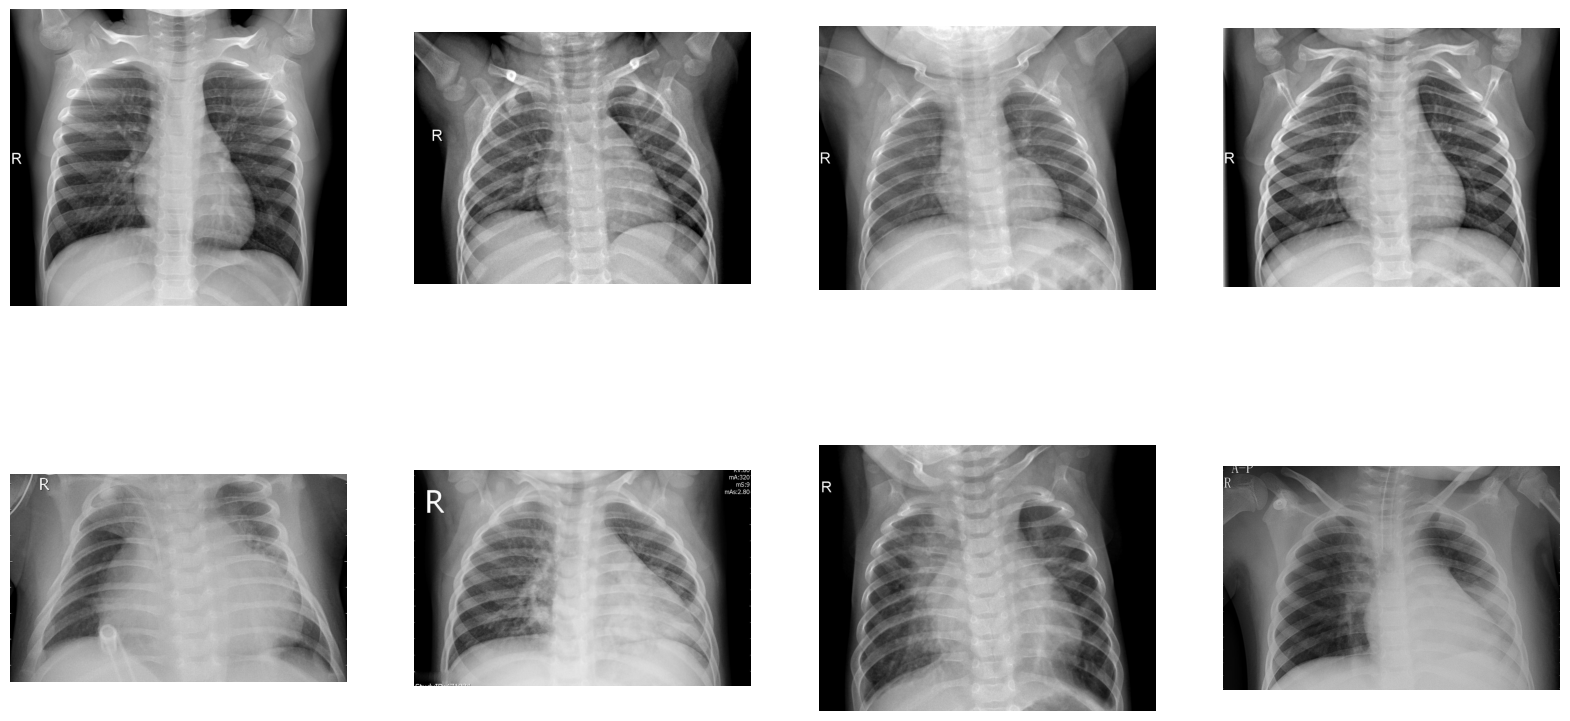
\includegraphics[width=1\textwidth]{images/samples.png}
    \end{subfigure}
    \caption{Visualization of X-rays from normal (upper row) and pneumonia (bottom row) class.}
    \label{fig:samples}
\end{figure}
Clearly, the lungs of sick patients appear more opaque (oftentimes in an asymmetric way), while the lungs of healthy patients appear more transparent/black (and equally so on both sides). In addition, the airways seem more pronounced and visible in sick patients.

A first problem becomes apparent when looking at Figure \ref{fig:samples}: the input sizes of the images are inconsistent. In addition, although not immediately apparent, some images are saved in 3-dimensional format, while others are saved as 2-dimensional images. We take this into account in all subsequent tasks by simply averaging the RGB values into a single grayscale value.

\subsection{Data Exploration}
For further data exploration, we first plot the average contrast distribution of all images in a histogram, and compare the resulting histograms between both classes. We expect images classified as 'pneumonia' to obtain slightly more bright values, due to the previously mentioned increased opaqueness of the lungs.
In addition, since input sizes are not homogeneous, we extract the image sizes and check if these are consistent between the two classes.
Finally, we apply principal component analysis (PCA) and check for consistency between train, validation, and test set.
Note that we normalize the image intensity for each image in order to allow for proper comparison between the different contrast windows used in X-ray imaging.

\begin{figure}[H]
    \centering
    \begin{subfigure}{\columnwidth}
        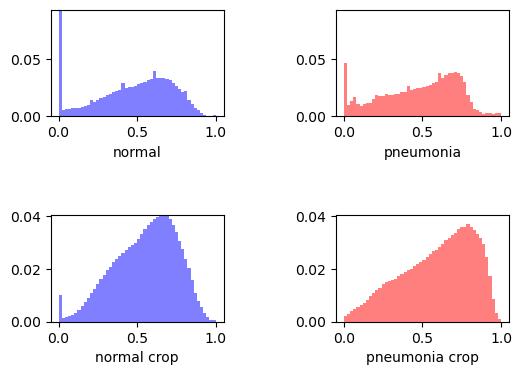
\includegraphics[width=1\textwidth]{images/histo_crop.png}
    \end{subfigure}
    \caption{Distribution of image intensities on a subset of cropped and non-cropped images.}
    \label{fig:histo_crop}
\end{figure}

\subsubsection{Histogram}
Due to the sheer size of some of the images, we check if cropping a subset of the images greatly affects the prominent features in the histogram. If not, we apply cropping for all further data analysis to prevent a needless increase in computation time.

As you can see in Figure \ref{fig:histo_crop}, although the histograms between cropped and non-cropped images are clearly different (the crop mostly removes black parts), the same trends can still be seen: the initial peak at intensity 0 (black) is higher in the normal samples, while the pneumonia samples show a peak at higher intensities than the normal samples. We deem these similarities to be important enough and therefore apply center-cropping to the images in all subsequent tasks.

\begin{figure}[H]
    \centering
    \begin{subfigure}{0.9\columnwidth}
        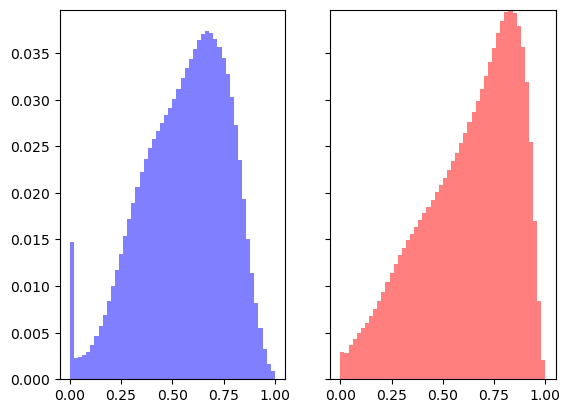
\includegraphics[width=1\textwidth]{images/histo.png}
    \end{subfigure}
    \caption{Distribution of image intensities over the entire dataset. Patients with pneumonia (red) have a peak at brighter values when compared to those without pneumonia (blue).}
    \label{fig:histo}
\end{figure}


If we now compare histograms obtained from the entire dataset, like in Figure \ref{fig:histo}, we can still see that samples with pneumonia seem to have brighter values in general, which makes sense, since one of the radiological features of pneumonia is an increase in visible tissue (visible due to inflammation and infection of the airways and lung parenchyma, but also due to fluid build ups) and the occurence of pleural effusions. Tissue and fluid are typically able to absorb more x-rays than air (which in contrast allows them to simply pass through), and therefore appear whiter on the X-ray image.

\subsubsection{Image Sizes}
Second, we visualize whether both classes have similar image sizes present. This might influence the cropping results (e.g. if all images in the 'normal' class have to be upsampled, while all images in the 'pneumonia' class should be downsampled, we might accidentally create a bias between the datasets).

\begin{figure}[H]
    \centering
    \begin{subfigure}{0.9\columnwidth}
        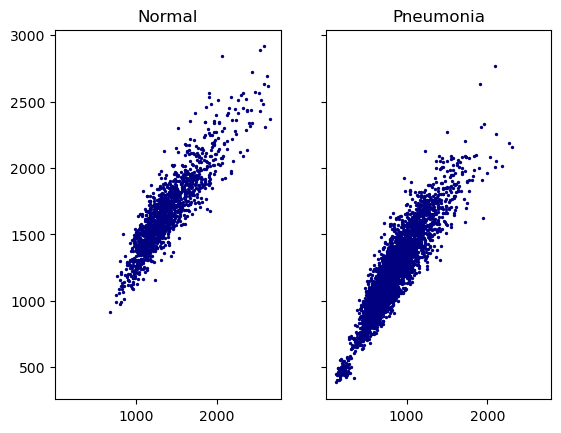
\includegraphics[width=1\textwidth]{images/sizes.png}
    \end{subfigure}
    \caption{Plot of image sizes per class. Height on y-axis, width on x-axis.}
    \label{fig:sizes}
\end{figure}

As can be seen in Figure \ref{fig:sizes}, image sizes vary widely, and images in the pneumonia class tend to have smaller sizes. We could make our model more robust to this by randomly zooming in/out on images and then resizing to the correct size. However, this could still cause a data bias, since images of patients with pneumonia will generally be zoomed into more if the size of the image is related to earlier cropping applied before adding the image to the dataset (and this seems to be the case). In addition, using the entire image as input for preprocessing will significantly decrease training speed. We therefore opt to only work with already center-cropped images.

\subsubsection{PCA}
Finally, we apply PCA to the cropped and normalized images in order to see whether there is a distinction between the two classes. We also compare with (but do not fit on) the validation and test set.

Figure \ref{fig:PCA} shows us that the main components are similarly distinct for train and test data, although there does seem to be more overlap for the test data.

\begin{figure*}
    \centering
    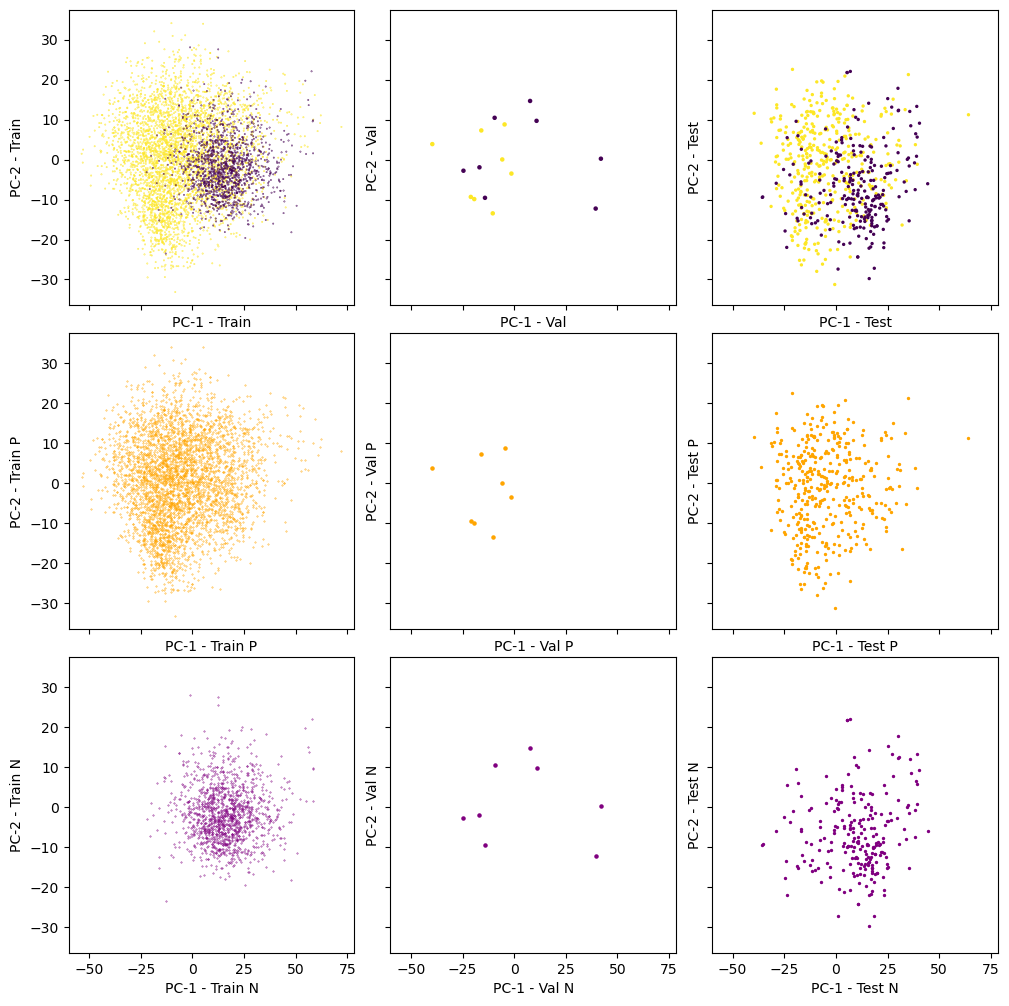
\includegraphics[width=0.8\textwidth]{images/PCA.png}
    \caption{Plot based on first two components of PCA. Upper row shows results for both classes in the same plot. Bottom two rows show them for each class separately. (orange: pneumonia, purple: normal).}
    \label{fig:PCA}
\end{figure*}
